
\section{結果}
\subsection{コマンドの命名原則}
機能ごとの動作はコマンドのオプションによって指定されます.
このオプションにどのような名前をつけるかは,どれだけコマンドを覚えやすいかという
意味で重要です.コマンドの振る舞いを的確に表す名称をつける必要があります.

この振る舞いとしてもっとも受け入れやすいのがshellで用意されているコマンドです.
pwd, ls, rm, touch, openなどはもっとも直感的に動作がわかるコマンドです.
hikiutilsの振る舞いを予測できるシェルコマンドと同じ名前でオプションを提供する
ようにします.

\subsubsection{hikiutilsの想定利用形態}
ここでhikiutilsがあらかじめ想定している利用形態を解説しておきます.

\begin{figure}[htbp]\begin{center}
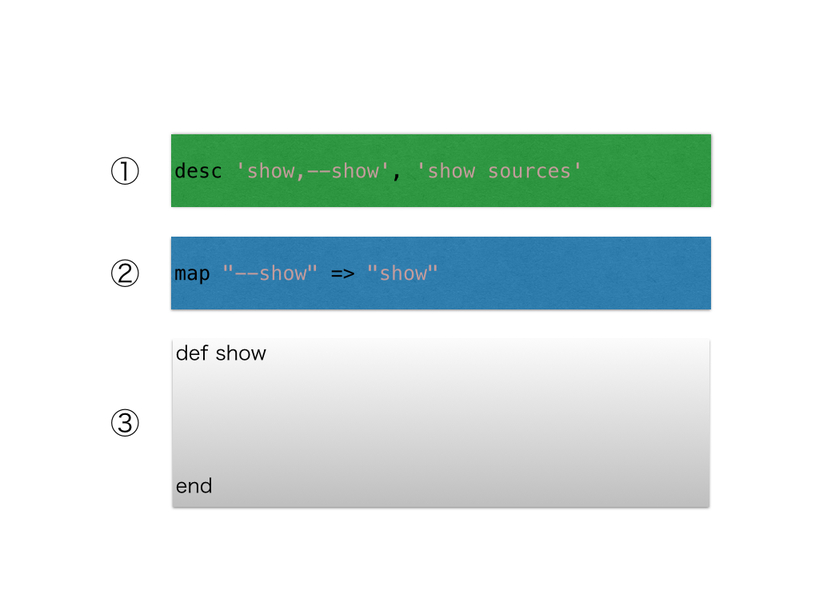
\includegraphics[width=10cm,bb= 0 0 737 553]{../figs/./hikiutils_yamane.002.jpg}
\caption{hikiutilsがあらかじめ想定している利用形態.}
\label{fig:002}
\label{default}\end{center}\end{figure}
hikiutilsは,

\begin{itemize}
\item local PCとglobal serverとが用意されており,
\item それらのデータをrsyncで同期する
\end{itemize}
ことで動作することを想定しています.これは,ネットに繋がっていないオフラインの状況でも
テキストなどの編集が可能で,さらに不用意な書き換えを防ぐための機構です.さらに,
どちらもが何かあった時のバックアップともなって,ミスによる手戻りを防いでいます.

これらの設定は,~/.hikircにyaml形式で記述・保存されています.
\begin{lstlisting}[style=,basicstyle={\scriptsize\ttfamily}]
bob% cat ~/.hikirc
:srcs:
- :nick_name: new_ist
  :local_dir: "/Users/bob/Sites/new_ist_data/ist_data"
  :local_uri: http://localhost/ist
  :global_dir: nishitani@ist.ksc.kwansei.ac.jp:/home/nishitani/new_ist_data/ist_data
  :global_uri: http://ist.ksc.kwansei.ac.jp/~nishitani/
- :nick_name: dmz0
  :local_dir: "/Users/bob/Sites/nishitani0/Internal/data"
  :local_uri: http://localhost/~bob/nishitani0/Internal
  :global_dir: bob@dmz0:/Users/bob/Sites/nishitani0/Internal/data
  :global_uri: http://nishitani0.kwansei.ac.jp/~bob/nishitani0/Internal
\end{lstlisting}
また,一般的に一人のユーザがいくつものまとまりとしてのlocal-globalペアを
保持して管理することが普通です.それぞれにnicke\_nameをつけて管理しています.
\begin{lstlisting}[style=,basicstyle={\scriptsize\ttfamily}]
bob% hiki -s
hikiutils: provide utilities for helping hiki editing.
"open -a mi"
target_no:1
editor_command:open -a mi
 id | name      | local directory                           | global uri     
-----------------------------------------------------------------------------
  0 | new_ist   | /Users/bob/Sites/new_ist_data/ist_data    | http://ist.ksc.k
 *1 | dmz0      | /Users/bob/Sites/nishitani0/Internal/data | http://nishitani
  2 | ist       | /Users/bob/Sites/hiki-data/data           | http://ist.ksc.k
  3 | new_maple | /Users/bob/Sites/new_ist_data/maple_hiki_d| http://ist.ksc.k
\end{lstlisting}
とすると,それらの一覧と,いまtargetにしているnick\_nameディレクリが表示されます.

\subsubsection{コメンド名と振る舞いの詳細}
検討の結果コマンドを以下のように書き換えることとします.
上部に記した,特によく使うコマンドに関しては,shellでよく使われるコマンド名と一致するにようにしました.

\begin{table}[htbp]\begin{center}
\caption{}
\begin{tabular}{llll}
\hline
変更前  &変更後  &動作の解説  \\ \hline
edit FILE         &open  &open file  \\
list [FILE]       &ls  &list files  \\
rsync             &rsync  &rsync files  \\
update FILE       &touch  &update file  \\
show              &pwd  &show nick\_names  \\
target VAL        &cd  &targetを変える,cdとのメタファ  \\
  &  \\
move [FILE]       &mv  &move file  \\
remove [FILE]     &rm  &remove files  \\
add               &  &add sources info  \\
checkdb           &  &check database file  \\
datebase FILE     &db  &read datebase file  \\
display FILE      &show  &display converted hikifile  \\
euc FILE          &  &translate file to euc  \\
help [COMMAND]    &-h  &Describe available commands  \\
version           &-v  &show program version  \\
\hline
\end{tabular}
\label{default}
\end{center}\end{table}
%for inserting separate lines, use \hline, \cline{2-3} etc.

それぞれの意図を動作の解説として記述しています.

\paragraph{open FILE}
ファイルを編集のためにeditorでopen.Editorは~/.hikircに
\begin{quote}\begin{verbatim}
:editor_command: open -a mi
\end{verbatim}\end{quote}
として保存されている.open -a miをemacsなどに適宜変更して使用.

\paragraph{ls [FILE]}
local\_dirにあるファイル名を[FILE*]として表示.例えば,hikiutils\_yamane以下の拡張子が
ついたファイルを表示.hikiシステムではtextディレクトリーは階層構造を取ることができない.
西谷研ではdirectoryの代わりにスネーク表記で階層構造を表している.

\paragraph{rsync}
local\_dirの内容をglobal\_dirにrsyncする.逆方向は同期に誤差が生じたり,permissionが
おかしくなるので,現在のところ一方向の同期のみとしている.したがって,作業手順としては
テキストの変更はlocal\_dirで読み行うようにしている.

\paragraph{touch FILE}
loccal\_dirで書き換えたFILEの内容をlocal\_uriに反映させ,ブラウザで表示.シェルコマンドの
touchによって,変更時間を現在に変え,最新状態とするのに似せてコマンド名をtouchとしている.

\paragraph{pwd}
nick\_nameの一覧とtargetを表示,current targetをcurrent dirとみなして,
コマンド名をpwdとした.

\paragraph{cd VAL}
targetを変える,change directoryとのメタファ.ただし,いまのところnick\_nameでは
対応しておらず,nick\_nameの番号をVAL入力することで変更する.

\subsection{Thorによる実装}
手法のところで概観した通り,thorを用いることで記述の簡略化が期待できる.ここでは,実際に書き換える前後,すなわちoptparse版とthor版の対応するコードを比較することで,以下の具体的な違い

\begin{itemize}
\item クラス初期化
\item コマンド定義
\item CLIの実行プロセス
\end{itemize}
について詳しく検討を行う.

\subsubsection{クラス初期化}
\begin{figure}[htbp]\begin{center}
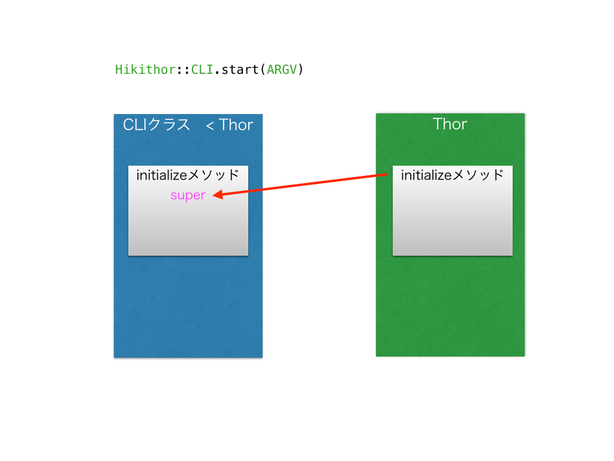
\includegraphics[width=10cm,bb= 0 0 737 553]{../figs/./hikiutils_yamane.003.jpg}
\caption{Thorのinitializeでのコード}
\label{default}\end{center}\end{figure}
Thorのinitializeでのコードはつぎの通りである.

\begin{enumerate}
\item Hikithor::CLI.start(ARGV)が呼ばれる
\item initializeメソッドが呼ばれる
\item これではThorのinitializeメソッドが呼ばれない
\item superを書くことでThorのinitializeメソッドが呼ばれる
\end{enumerate}
optparseではrequireでoptparseを呼びoptparseのinitializeを定義する必要はないが,Thorはinitializeを定義する必要がある.Thorの定義方法はrequireでThorを呼びCLIクラスで継承し,initializeメソッドにsuperを書くことでThorのinitializeが呼ばれる.initializeメソッド内ではThorの初期設定がされていないため,スーパークラスのメソッドを読み出してくれるsuperを書き加えることで図のようにinitializeメソッド内でThorのinitilalizeメソッドが呼ばれ定義される.
\begin{lstlisting}[style=customRuby,basicstyle={\scriptsize\ttfamily}]

module Hikithor

  DATA_FILE=File.join(ENV['HOME'],'.hikirc')
  attr_accessor :src, :target, :editor_command, :browser, :data_name, :l_dir

  class CLI < Thor
   def initialize(*args)
      super
      @data_name=['nick_name','local_dir','local_uri','global_dir','global_uri']
      data_path = File.join(ENV['HOME'], '.hikirc')
      DataFiles.prepare(data_path)

      ...以下略...
   end
\end{lstlisting}
\subsubsection{コマンド定義}
\begin{figure}[htbp]\begin{center}
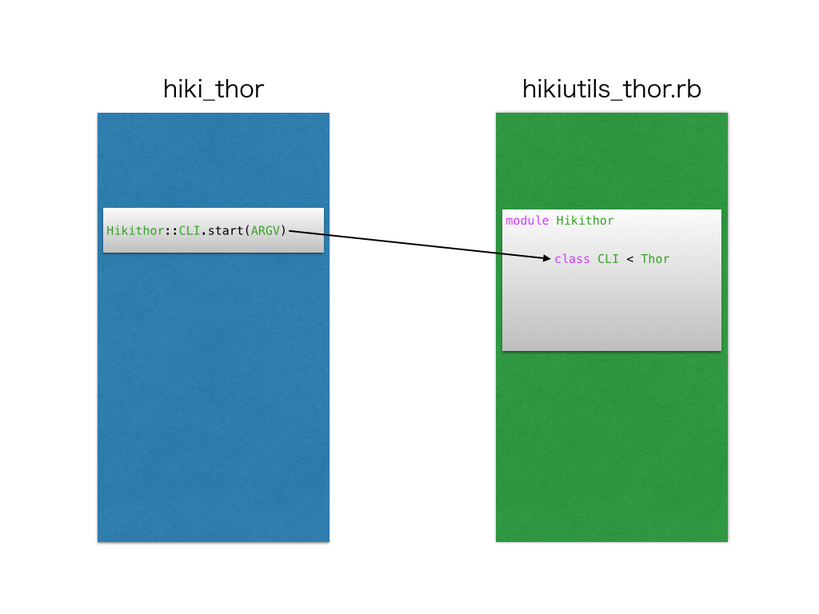
\includegraphics[width=10cm,bb= 0 0 737 553]{../figs/./hikiutils_yamane.004.jpg}
\caption{thorにおけるコマンド記述のひな形.}
\label{default}\end{center}\end{figure}
thorではoptparseのような登録処理はない.図にある通りにコマンドが記述され,それらは以下のように構成される.

\begin{enumerate}
\item desc以降にコマンド名と,その説明が記述される.これらはコマンドhelpで一覧として表示させる
\item mapによって別のコマンド名でも実行できるように定義される.
\item defで定義されたメソッドの実行コード
\end{enumerate}
Thorではdescで一覧を表示されるコマンド名,コマンドの説明を登録する.しかし,ここで記述したコマンドは単に一覧で表示させるためのものであり,実際に実行される時に呼び出すコマンド名は,defで定義された名前である.Thorでは処理実行を行うメソッド名がコマンド名となり,コマンド名1つが対応する.

これに別名を与えるために利用されるキーワードがmapである.
\begin{quote}\begin{verbatim}
map A => B
\end{verbatim}\end{quote}
mapとはBと呼ばれるメソッドをAでも呼べるようにしてくれるものである.
よって,これを使うことでコマンドの別名を指定することができる.
\begin{lstlisting}[style=customRuby,basicstyle={\scriptsize\ttfamily}]
    desc 'show,--show', 'show sources'
    map "--show" => "show"
    def show
      printf("target_no:%i\n",@src[:target])
      printf("editor_command:%s\n",@src[:editor_command])
      ,,,以下略...
    end
\end{lstlisting}
以上より,Thorではコマンドの指定と処理にはdesc,map,処理メソッドだけで済む.optparseではコマンドを登録するためのメソッドと処理メソッドの両方が必要になっていた.一方Thorでは,処理メソッドが直接コマンド名となるため記述が簡潔になる.

\subsubsection{CLIの実行プロセス}
\begin{figure}[htbp]\begin{center}
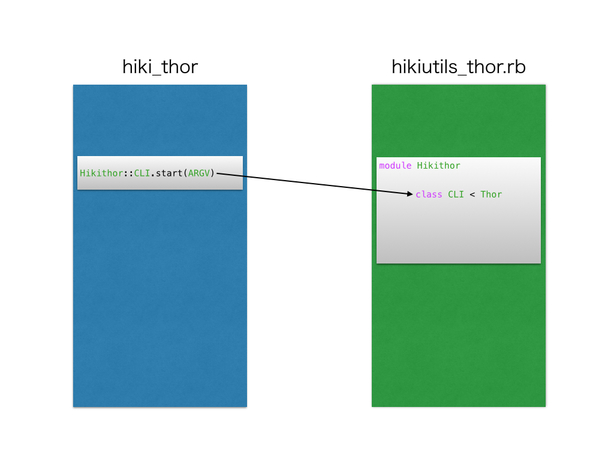
\includegraphics[width=10cm,bb= 0 0 737 553]{../figs/./hikiutils_yamane.006.jpg}
\caption{CLIの実行プロセス.}
\label{default}\end{center}\end{figure}
Thorにおけるcliの実行プロセスは次の通りである.

\begin{enumerate}
\item hiki\_thorのHikithor::CLI.start(ARGV)でhikiutils\_thor.rbのCLIクラスを呼ぶ
\item hikiutils\_thor.rbのCLIクラスのメソッドを順に実行していく
\end{enumerate}
Thorではstart(ARGV)を呼び出すことでCLIを開始する.Hikithor::CLI.start(ARGV)を実行されることによりrequireで呼ばれているhikiutils\_thor.rbのCLIコマンドを順に実行する.そして,入力されたコマンドと一致するメソッドを探し,そのコマンドの処理が実行される.
\begin{lstlisting}[style=customRuby,basicstyle={\scriptsize\ttfamily}]
#!/usr/bin/env ruby                                                             

require "hikiutils_thor"

Hikithor::CLI.start(ARGV)
\end{lstlisting}\begin{lstlisting}[style=customRuby,basicstyle={\scriptsize\ttfamily}]

module Hikithor

  DATA_FILE=File.join(ENV['HOME'],'.hikirc')
  attr_accessor :src, :target, :editor_command, :browser, :data_name, :l_dir

  class CLI < Thor
   def initialize(*args)
      super
      @data_name=['nick_name','local_dir','local_uri','global_dir','global_uri']
      data_path = File.join(ENV['HOME'], '.hikirc')
      DataFiles.prepare(data_path)
      ...以下略...
\end{lstlisting}
Thorではクラスのメソッドを順に実行していくためrunメソッドとexecuteメソッドは必要ない.
また,optparseでの実行手順はメソッドの移動回数が多く複雑であるが,Thorは単純で分かりやすいものとなっている.

\subsubsection{optparseとの全体的な比較}
Thorとoptparseでのコードの違いは以上の部分になるが,コードからもThorのほうが短くなっていることが分かる.
しかし,Thorの問題点はメソッド名がコマンドとなるため,1つしか定義できないことである.
これを解決するためにmapを用い,複数のコマンドを定義できるようにした.
一方,optparseでは別のコマンドを定義するにはfizzbuzzのoptparseのコードで解説したやり方になる.
よって,全体的にもThorのほうがコードが短くなり,コマンドの定義も簡単に行うことができる.
また,実行手順も分かりやすくコードが読みやすいため書き換えもすぐ行うことができるので,より直感的なコマンドを実装することも可能となった.

